\documentclass[11pt,epsf]{article}
\usepackage{amsmath,amsfonts}
\usepackage{amsthm,amssymb,hyperref}
\usepackage{tikz}
\usepackage{pgfplots}
\usepackage{pgfplotstable}
\usepackage{tikzscale}
\usetikzlibrary{decorations.markings}
\usetikzlibrary{shapes}
\usetikzlibrary{arrows}

\begin{document}

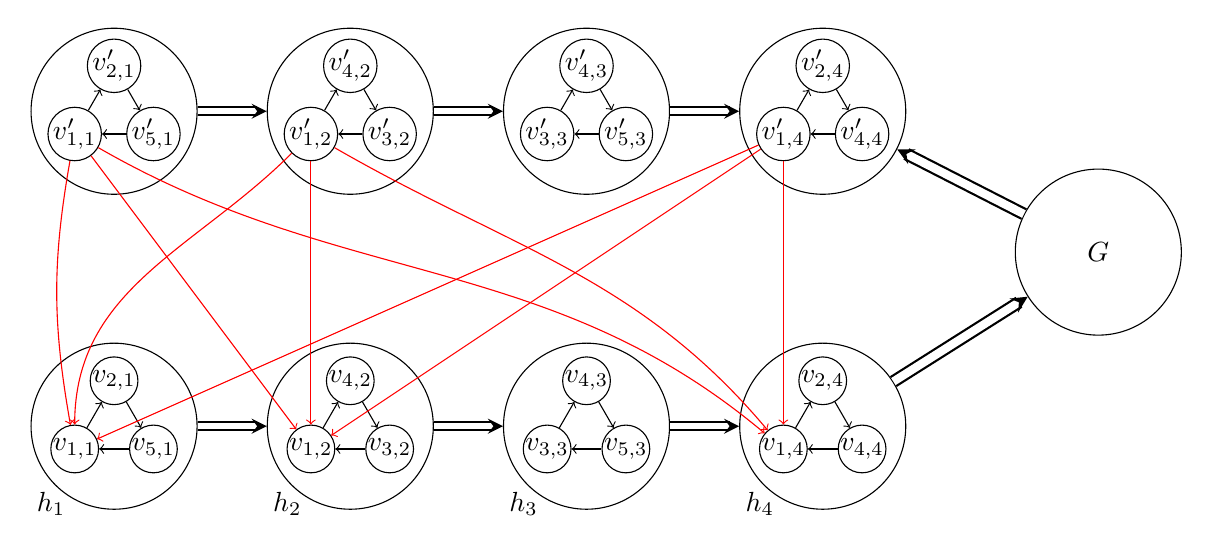
\begin{tikzpicture}
	  % define vertex styles
	  \tikzstyle{smallvertex}=[circle,draw,minimum size=10pt,inner sep=0pt]
	  \tikzstyle{bigvertex}=[circle,draw,minimum size=40pt,inner sep=0pt]
	  \tikzstyle{group}==[circle,draw,minimum size=60pt,inner sep=0pt]

  	  % draw vertices
	  \node[smallvertex] (v1) at (0,0) {$v_{1,1}$};
	  \node[smallvertex] (v2) at (0.5,0.866) {$v_{2,1}$};
	  \node[smallvertex] (v3) at (1,0) {$v_{5,1}$};
	  \node[group] (g1) at (0.5,0.289) {$$};
	  \node at (-0.3,-0.7) {$h_1$};
	  % draw edges
	  \draw [->] (v1) to (v2);
	  \draw [->] (v2) to (v3);
	  \draw [->] (v3) to (v1);

	  \begin{scope}[xshift=3cm]
	  % draw vertices
	  \node[smallvertex] (v4) at (0,0) {$v_{1,2}$};
          \node[smallvertex] (v5) at (0.5,0.866) {$v_{4,2}$};
          \node[smallvertex] (v6) at (1,0) {$v_{3,2}$};
          \node[group] (g2) at (0.5,0.289) {$$};
	  \node at (-0.3,-0.7) {$h_2$};
          % draw edges
          \draw [->] (v4) to (v5);
          \draw [->] (v5) to (v6);
          \draw [->] (v6) to (v4);
	  \end{scope}

          \begin{scope}[xshift=6cm]
          % draw vertices
          \node[smallvertex] (v7) at (0,0) {$v_{3,3}$};
          \node[smallvertex] (v8) at (0.5,0.866) {$v_{4,3}$};
          \node[smallvertex] (v9) at (1,0) {$v_{5,3}$};
          \node[group] (g3) at (0.5,0.289) {$$};
	  \node at (-0.3,-0.7) {$h_3$};
          % draw edges
          \draw [->] (v7) to (v8);
          \draw [->] (v8) to (v9);
          \draw [->] (v9) to (v7);
          \end{scope}

          \begin{scope}[xshift=9cm]
          % draw vertices
          \node[smallvertex] (v10) at (0,0) {$v_{1,4}$};
          \node[smallvertex] (v11) at (0.5,0.866) {$v_{2,4}$};
          \node[smallvertex] (v12) at (1,0) {$v_{4,4}$};
          \node[group] (g4) at (0.5,0.289) {$$};
	  \node at (-0.3,-0.7) {$h_4$};
          % draw edges
          \draw [->] (v10) to (v11);
          \draw [->] (v11) to (v12);
          \draw [->] (v12) to (v10);
          \end{scope}

	  % draw edges
	  \draw [->,>=stealth,thick,double distance=2pt] (g1) to (g2);
	  \draw [->,>=stealth,thick,double distance=2pt] (g2) to (g3);
	  \draw [->,>=stealth,thick,double distance=2pt] (g3) to (g4);

	  \begin{scope}[yshift=4cm]
          % draw vertices
          \node[smallvertex] (u1) at (0,0) {$v'_{1,1}$};
          \node[smallvertex] (u2) at (0.5,0.866) {$v'_{2,1}$};
          \node[smallvertex] (u3) at (1,0) {$v'_{5,1}$};
          \node[group] (h1) at (0.5,0.289) {$$};
          % draw edges 
          \draw [->] (u1) to (u2);
          \draw [->] (u2) to (u3);
          \draw [->] (u3) to (u1);

          \begin{scope}[xshift=3cm]
          % draw vertices
          \node[smallvertex] (u4) at (0,0) {$v'_{1,2}$};
          \node[smallvertex] (u5) at (0.5,0.866) {$v'_{4,2}$};
          \node[smallvertex] (u6) at (1,0) {$v'_{3,2}$};
          \node[group] (h2) at (0.5,0.289) {$$};
          % draw edges 
          \draw [->] (u4) to (u5);
          \draw [->] (u5) to (u6);
          \draw [->] (u6) to (u4);
          \end{scope}

          \begin{scope}[xshift=6cm]
          % draw vertices
          \node[smallvertex] (u7) at (0,0) {$v'_{3,3}$};
          \node[smallvertex] (u8) at (0.5,0.866) {$v'_{4,3}$};
          \node[smallvertex] (u9) at (1,0) {$v'_{5,3}$};
          \node[group] (h3) at (0.5,0.289) {$$};
          % draw edges 
          \draw [->] (u7) to (u8);
          \draw [->] (u8) to (u9);
          \draw [->] (u9) to (u7);
          \end{scope}

          \begin{scope}[xshift=9cm]
          % draw vertices
          \node[smallvertex] (u10) at (0,0) {$v'_{1,4}$};
          \node[smallvertex] (u11) at (0.5,0.866) {$v'_{2,4}$};
          \node[smallvertex] (u12) at (1,0) {$v'_{4,4}$};
          \node[group] (h4) at (0.5,0.289) {$$};
          % draw edges 
          \draw [->] (u10) to (u11);
          \draw [->] (u11) to (u12);
          \draw [->] (u12) to (u10);
          \end{scope}

          % draw edges
          \draw [->,>=stealth,thick,double distance=2pt] (h1) to (h2);
          \draw [->,>=stealth,thick,double distance=2pt] (h2) to (h3);
          \draw [->,>=stealth,thick,double distance=2pt] (h3) to (h4);
	  \end{scope}


	  \node[group] (G) at (13,2.5) {$G$};

	  % draw edges
          \draw [->,>=stealth,thick,double distance=3pt] (g4) to (G);
          \draw [->,>=stealth,thick,double distance=3pt] (G) to (h4);
          \draw [->,red, out=-100, in=100] (u1) to (v1);
          \draw [->,red, out=-135, in=90] (u4) to (v1);
          \draw [->,red] (u10) to (v1);
          \draw [->,red] (u1) to (v4);
          \draw [->,red] (u4) to (v4);
          \draw [->,red] (u10) to (v4);
          \draw [->,red, out = -30, in = 140] (u1) to (v10);
          \draw [->,red, out = -30, in = 130] (u4) to (v10);
          \draw [->,red] (u10) to (v10);



\end{tikzpicture}

\end{document}